\PassOptionsToPackage{english,ngerman}{babel}
\documentclass[course=erap]{aspdoc}
%aspdoc%
%eigentlich ist es kein article sondern ein aspdoc, aber aspdoc wirft einen fehler%

\usepackage{subfigure}
\usepackage{hyperref}
\usepackage{amsmath}
\usepackage{graphicx}
\usepackage{listings}
\usepackage{xcolor}
\lstset{
  basicstyle=\ttfamily,
  columns=fullflexible,
  breaklines=true,
  postbreak=\raisebox{0ex}[0ex][0ex]{\color{red}$\hookrightarrow$\space}
}

\graphicspath{ {./images/} }
\newcommand{\theGroup}{114}
\newcommand{\theNumber}{A305}
\author{Daniel Petri Rocha \and Dominik Fuchs \and Robin Geißler}
\date{Wintersemester 2018/19}

\title{Gruppe \theGroup{} -- Abgabe zu Aufgabe \theNumber}

\begin{document}
\maketitle

\tableofcontents







\section{Einleitung}

Im Zuge des Rechnerarchitektur Praktikums wurde sich das Ziel gesetzt, das Wissen, das wir uns während des Rechnerarchitektur-Moduls im ersten Semester angeeignet haben, zu vertiefen. Dazu gehörte in erster Linie das Kennenlernen der 64 Bit Register - denn bisher wurde in der Rechnerarchitektur Vorlesungen maximal mit 32 Bit Registern gearbeitet - und das Arbeiten mit Calling Conventions.\\ Den Großteil der Vorbereitungszeit nahmen die so genannten SIMD-Instruktionen (Single Instruction Multiple Data) in Anspruch. Die im Tutorium besprochenen Befehle arbeiten auf 128 Bit Registern, und ermöglichen es, 4 32-bit Operationen parallel durchzuführen. Die Befehle dafür wurden in den SSE Erweiterungen eingeführt, von denen wir uns mit den ersten beiden - SSE für Single Precision Befehle und SSE2 für Double Precision Befehle - beschäftigt haben.\\
In den letzten beiden Wochen der Vorbereitungszeit wurde das Augenmerk auf die Sicherheit von Assembler und C Programmen, sowie auf Laufzeitmessungen gerichtet. Die Security und Performance sind Aspekte, die auch wir in unserer Ausarbeitung betrachten. Die Vorbereitungszeit war also eine notwendige und sehr hilfreiche Einarbeitung in die Themen mit denen wir uns in unserem Projekt beschäftigen.


\section{Problemstellung und Spezifikation}

Die Aufgabenstellung ist unterteilt in die Konzeption - den theoretischen Teil - und die Implementierung des Programms - den praktischen Teil. 

\subsubsection{Konzeptioneller Teil}

Im konzeptionellen Teil sollen die Newton-Cotes Formeln für n = 1 und n = 2 von Hand berechnet, und so weit wie möglich vereinfacht werden. Die Umformung soll so erfolgen, dass danach nur noch die vier Grundrechenarten (Addition, Subtraktion, Multiplikation, Division), sowie die Variablen a, b (Integrationsgrenzen) und die Stützstellen p{\tiny n} verwendet werden.\\
Mithilfe von Integrationsregeln soll folgende Formel in die so genannte abgeschlossene Newton-Cotes Formel gebracht werden, welche die ausschließliche Benutzung von Grundrechenarten impliziert:
\begin{equation}
[f] = \int_{a}^{b} p(x) dx = (b-a) * \sum_{i=0}^{n} \alpha_{in} * p(x_i)
\end{equation}
wobei darüber hinaus noch gegen ist, dass $x_i$ dargestellt wird durch
\begin{equation}
x_i = a + \frac {i * (b-a)}{n}
\end{equation} 
und für die Gewichte $\alpha_{in}$ gilt: 
\begin{equation}
\alpha_{in} = \frac{1}{n} \int_{0}^{n} \prod_{j= 0\atop j \neq i}^{n}\quad \frac{x-j}{i-j}
\end{equation}
Die Aufgabenstellung forderte uns außerdem auf, uns über folgenden Themen zu informieren 
\begin{enumerate}
\item korrekte Verwendung von Funktionspointern in C
\item Verwendung/Einbindung dynamischer Bibliotheken in C und Assembler
\end {enumerate}
Es soll zudem analysiert werden, wie nah die Werte der Annäherungen dem des eigentlichen Integrals kommen und wie es um die Programmsicherheit steht.

\subsubsection{Implementierung}

Zu implementieren sind zwei Funktionen:
\begin{enumerate}
\item float *newton\_cotes\_1(float (*p)(float), int a, int b)
\item double *newton\_cotes\_2(double(*p)(double), int a, int b)
\end{enumerate}
Newton\_cotes\_1 soll das Ergebnis der numerischen Quadratur nach der Newton-Cotes Formel mit n = 1 berechnen. Die Genauigkeit der Ein- und Ausgabe ist float. Das bedeutet, es muss mit single precision gerechnet werden. Zur Berechnung der Stützstellen soll die Funktion p, die im ersten Übergabeparameter übergeben wird, genutzt werden.\\
Newton\_cotes\_2 soll das Ergebnis der numerischen Quadratur nach der Newton-Cotes Formel mit n = 2 berechnen. Die Genauigkeit der Ein- und Ausgabe ist double. Das bedeutet, es muss mit double precision gerechnet werden. Zur Berechnung der Stützstellen soll auch hier die Funktion p, die im ersten Übergabeparameter übergeben wird, genutzt werden.\\
Darüber hinaus wird verlangt, ein Rahmenprogramm in C zu implementieren, das die beiden externen Funktionen newton\_cotes\_1 und newton\_cotes\_2 ausführt. Es soll vom Benutzer per Kommandozeile den Namen einer Funktion aus der Programmbibliothek übergeben bekommen, der dann zur Berechnung der Newton-Cotes Programme verwendet wird. Die eingebundene Bibliothek übergibt dann dem Programm die Funktion, die angefragt wurde. Diese Funktion hat die Form \glqq double f(double x)\grqq{}.\\
Zu guter Letzt soll ein Makefile geschrieben werden, das das Projekt durch den Aufruf von \glqq make\grqq{} vollständig kompiliert.

\section{Lösungsfindung}
\subsubsection{Lösungsfindung im Konzeptionellen Teil}

Die Berechnung der Newton-Cotes Formeln von Hand:
Zur händischen Berechnung der Newton-Cotes Formeln benötigt man grundlegende Kenntnisse über das Lösen von Integralen, sowie grundlegende mathematische Umformungen von Summation und Multiplikation.
Mit folgenden Schritten wurde die Newton-Cotes-Formel umgeformt, um die Abgeschlossene Newton-Cotes-Formel zu erreichen:\\
Newton-Cotes-Formel mit einer Stützstelle:
\begin{align*}
 I_1[f] &= \int_{a}^{b} p(x)dx = (b-a) * \sum_{i=0}^{1}\alpha_{i1} * p(x_i) \\
&= (b-a)*((\alpha_{01} * p(x_0))+(\alpha_{11} * p(x_1))\\
\end{align*}
Bestimmung der $x_i$ : 
\begin{align*}
x_0 = a + \frac{0*(b-a)}{1} = a\\
x_1 = a + \frac{1*(b-a)}{1} = b
\end{align*}
also:
\begin{align*}
(b-a)*(\alpha_{01}*p(a) + \alpha_{11}* p(b))
\end{align*}
Mit i = 0 gilt für die Gewichte :
\begin{align*}
\alpha_{01} &= 1*\int_{0}^{1}\prod_{j= 0\atop j \neq i}^{1} \frac{x-j}{i-j}dx = \int_{0}^{1} \frac{x-1}{-1} = \int_{0}^{1} 1-x = 0,5 \\
\alpha_{11} &= 1*\int_{0}^{1}\frac{x-0}{1-0} = \int_{0}^{1}x = 0,5
\end{align*}
damit:

\begin{align*}
I_1[f]&= (b-a)*(0,5*p(a) + 0,5*p(b))\\
&= (b-a)* \frac{p(a)+p(b)}{2}\\
&= Trapezformel
\end{align*}\\
Newton-Cotes-Formel mit zwei Stützstellen:
\begin{align*}
I_2[f] &= \int_{a}^{b}p(x) dx = (b-a)*\sum_{i=0}^{2}\alpha_{i2}*p(x_i)\\
&= (b-a)*(\alpha_{02}*p(x_0)+\alpha_{12}*p(x_1)+\alpha_{22}*p(x_2))
\end{align*}
Bestimmung der $x_i$:
\begin{align*}
x_0 &=a \\
x_1 &= a + \frac{(b-a)}{2} = \frac{2a + b - a}{2} = \frac{a+b}{2}\\
x_2 &= a + \frac{2*(b-a)}{2} = b
\end{align*}
Bestimmung der Gewichte:
\begin{align*}
\alpha_{02} &= \frac{1}{2}*\int_{0}^{2}\prod_{j= 0\atop j \neq i}^{2} \frac{x-j}{i-j}dx 
=\frac{1}{2}*\int_{0}^{2} \frac{x-1}{0-1} * \frac{x-2}{0-2} = \frac{1}{2}*\int_{0}^{2} \frac{x-1}{-1}*\frac{x-2}{-2}\\
&= \frac{1}{2}*\int_{0}^{2}\frac{(x-1)*(x-2)}{2} = \frac{1}{2}*\frac{1}{3} = \frac{1}{6}\\
\alpha_{12} &= \frac{1}{2}*\int_{0}^{2}\prod_{j= 0\atop j \neq i}^{2}\frac{x-j}{i-j} =\frac{1}{2} * \int_{0}^{2}(\frac{x}{1}*\frac{x-2}{1-2}) = \frac{1}{2}*\int_{0}^{2}\frac{x*(x-2)}{-1}\\
&= \frac{1}{2}*\int_{0}^{2}\frac{x^{2}-2x}{-1} = \frac{1}{2}*\int_{0}^{2} -x^{2}+2x = \frac{1}{2} * \frac{3}{4} = \frac{4}{6}\\
\alpha_{22} &= \frac{1}{2} * \int_{0}^{2}\prod_{j= 0\atop j \neq 2}^{2}\frac{x-j}{i-j}dx \\
&= \frac{1}{2}*\int_{0}^{2} (\frac{x}{2-0}*\frac{x-1}{2-1}) = \frac{1}{2}*\int_{0}^{2} (\frac{x}{2}*\frac{x-1}{1}) \\&= \frac{1}{2} * \int_{0}^{2} \frac{x*(x-1)}{2} = \frac{1}{2} * \int_{0}^{2} \frac{x^2-x}{2} = \frac{1}{2} * \frac{1}{3} = \frac{1}{6} \\
&\Rightarrow I_2[f] = (b-a)* (\frac{1}{6} * p(a)+\frac{4}{6} * p(\frac{a+b}{2}) + \frac{1}{6}*p(b)) \\
&= (b-a)*\frac{p(a) + 4*p(\frac{a+b}{2}) + p(b)}{6} = Keplersche\ Fassregel
\end{align*}
Als Ergebnis erhält man die so genannte abgeschlossene Newton-Cotes Formel, welche nur noch Grundrechenoperationen enthält und die im Anschluss implementiert werden soll.\\
Eine große Rolle spielt dabei das Einbinden von Funktionspointern in das Rahmenprogramm. Die Recherche diesbezüglich war relativ schnell abgeschlossen, da wir mit dieser Anwendung bereits in anderen Projekten gearbeitet haben. Um unser Wissen auf Korrektheit zu überprüfen, sowie zu vertiefen, haben wir die Thematik in dem Buch „C von A bis Z“ von „Jürgen Wolf“ nachgeschlagen.\\
\\
Bei der Recherche zur Verwendung und Einbindung dynamischer Bibliotheken haben wir hauptsächlich Artikel der Seite \url{https://eli.thegreenplace.net/} verwendet. Hier war besonders anschaulich und praxisnah erklärt wie die Einbindung von „Position Independent Code“ funktioniert. Besonders hilfreich war der Artikel mit dem Titel \hyperref[link1]{"Position Independent Code (PIC) in shared libraries"}.\\
\\
Im Nachfolgenden wird die grafische Ausarbeitung einiger im Test implementierten Funktionen aufgeführt. Die rote Linie stellt dabei die Ergebnisse von newton\_cotes\_2 dar, die orangene Linie die von newton\_cotes\_1. Um genaue Werte zu erhalten, benutze man das Flag $-t$ bei Programmausführung.\\




\begin{minipage}[t]{0.5\textwidth}
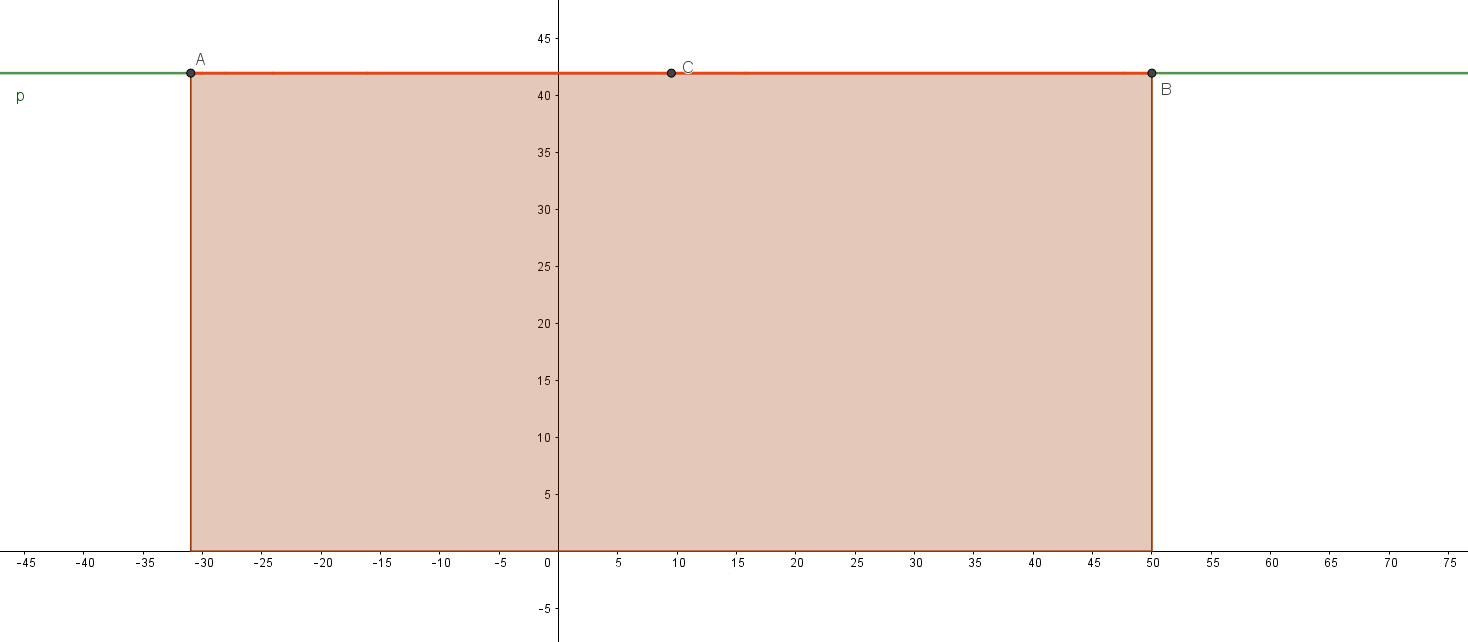
\includegraphics[width=0.9\textwidth]{42_-31_50}
$p(x) = 42$
\end{minipage}
\begin{minipage}[t]{0.5\textwidth}
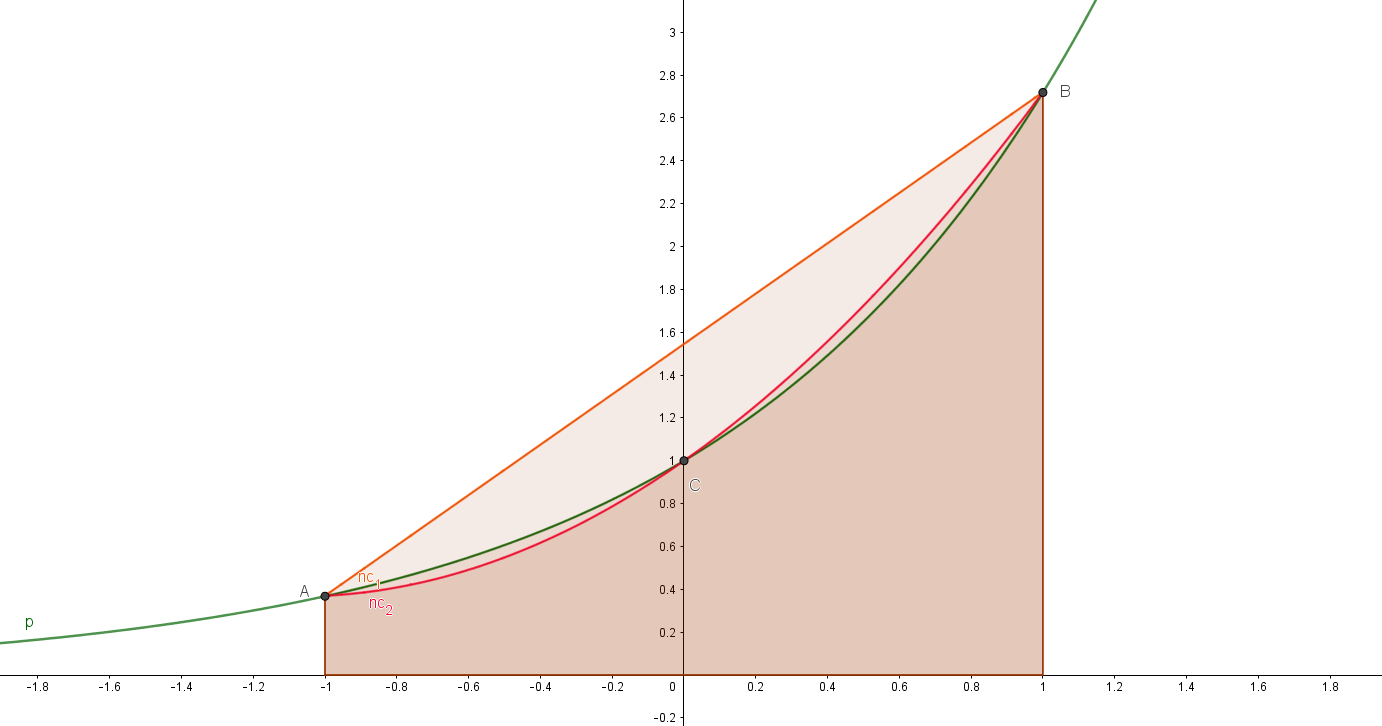
\includegraphics[width=0.9\textwidth]{e^x_-1_1}
$p(x) = e^x$
\end{minipage}\\
\\
\\\begin{minipage}[t]{0.5\textwidth}
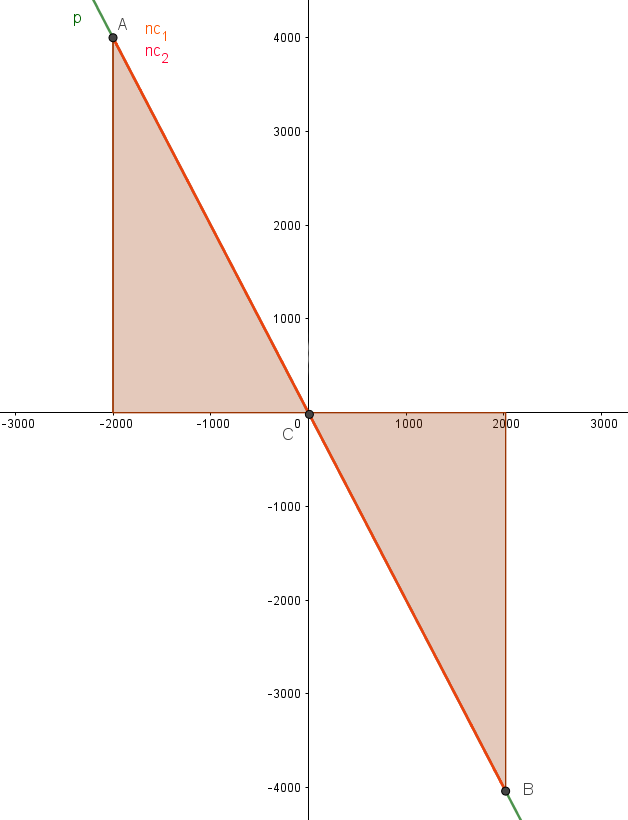
\includegraphics[width=0.9\textwidth]{min2x_-2000_-_2019}\\
$p(x) = -2x$\\
\end{minipage}
\begin{minipage}[t]{0.5\textwidth}
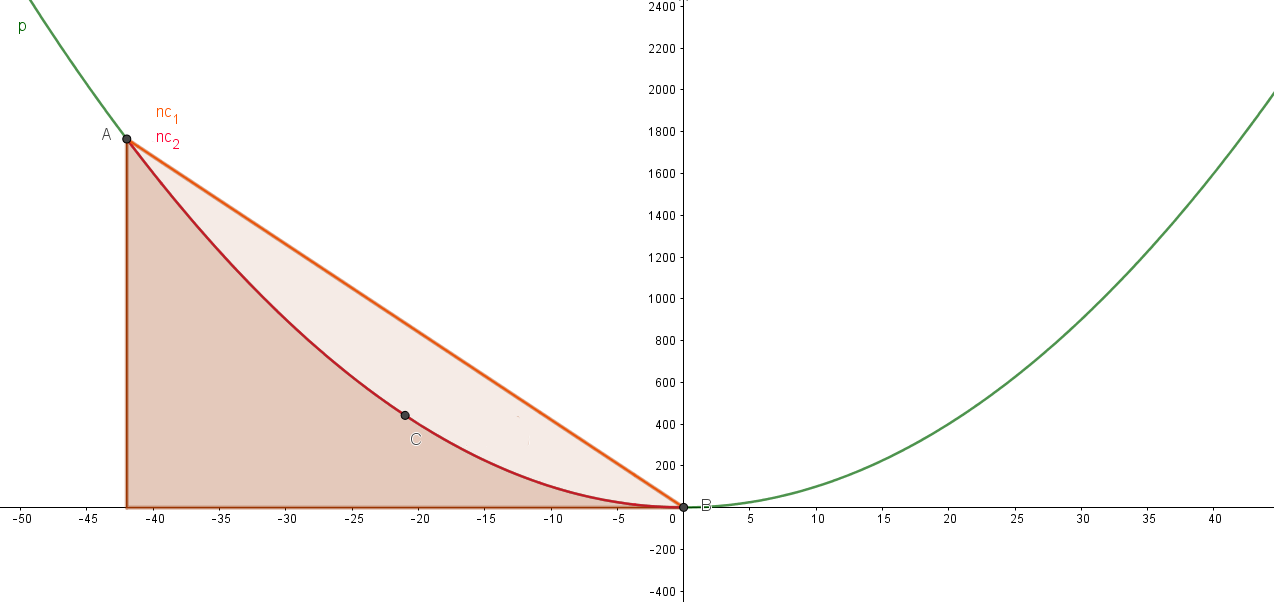
\includegraphics[width=0.9\textwidth]{x^2+1_-42_0}\\
$p(x) = x^2+1$\\
\end{minipage}\\
\begin{minipage}[t]{0.5\textwidth}
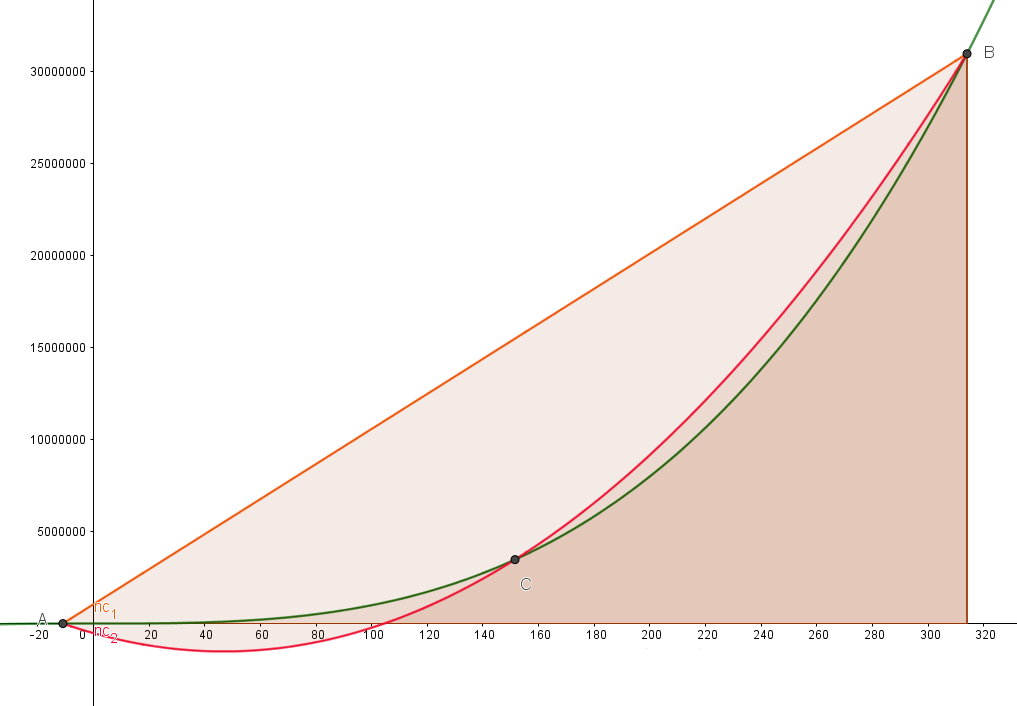
\includegraphics[width=0.9\textwidth]{x^3-25x_-11_314}\\
$p(x) = x^3-25x$\\
\end{minipage}
\begin{minipage}[t]{0.5\textwidth}
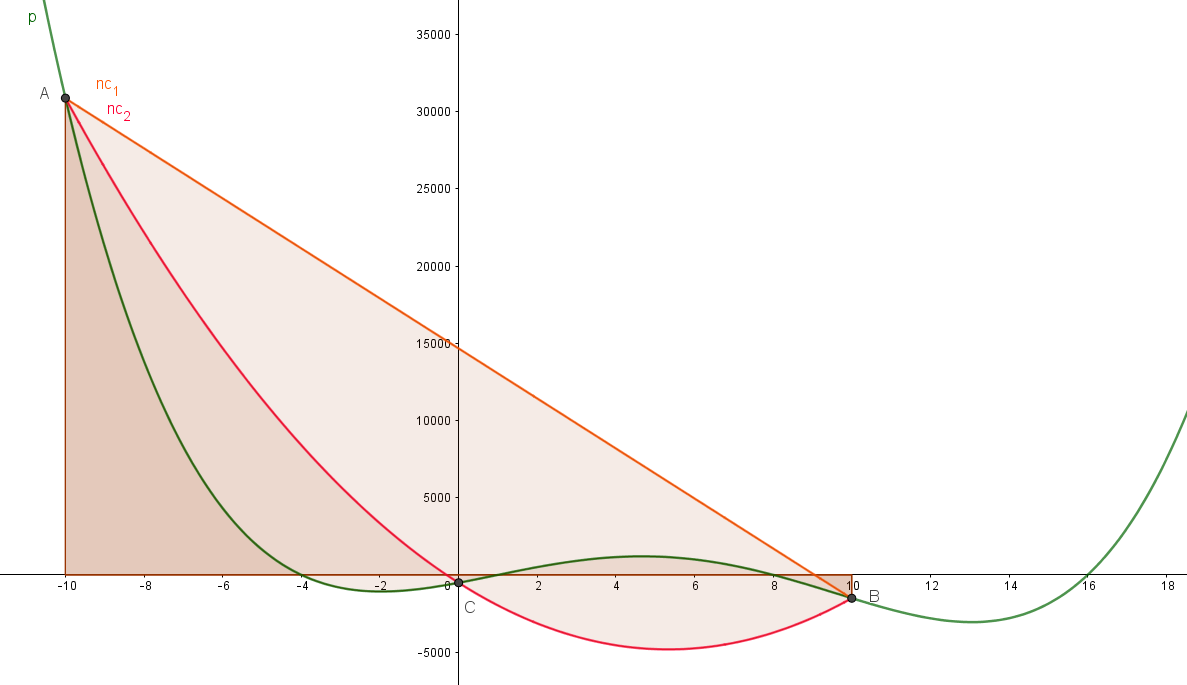
\includegraphics[width=0.9\textwidth]{x^4-21x^3+52x^2+480x-512_-10_10}\\
$p(x) = x^4-21x^3+52x^2+480x-512$\\
\end{minipage}\\
\\
\\\begin{minipage}[t]{0.5\textwidth}
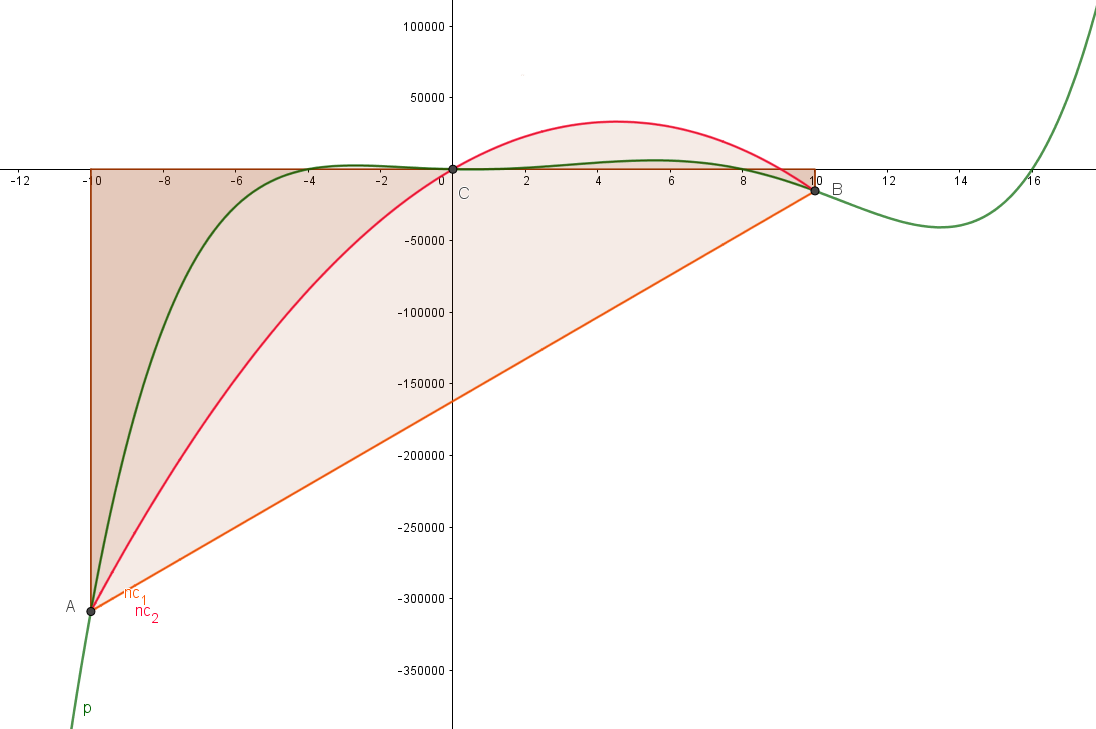
\includegraphics[width=0.9\textwidth]{x^5-21x^4+52x^3+480x^2-512x_-10_10}\\
$p(x) = x^5-21x^4+52x^3+480x^2-512x$\\
\end{minipage}

\subsection{Lösungsfindung während der Implementierung}
\subsubsection{C Rahmenprogramm}
Da die zu verwendenden Bibliotheken zur Compile-Zeit des Programms noch nicht verfügbar sind, werden sie erst zur Laufzeit eingebunden. \\
Um die Bibliothek dynamisch zu laden, bietet sich das Modul $dlfcn.h$ an. Dieser Header definiert die Methoden $void\ *dlopen(const\ char *,\ int)$ und  $void\ *dlsym(void *,\ const char *)$, die zusammen im Rahmenprogramm zulassen, dass der Benutzer das zu integrierende Funktion $p$ frei wählen kann.\\
Mit $void\ *dlopen(const\ char *, int)$ beispielsweise wird die übergebene Bibliothek geladen. Durch das Flag $RTLD\_LAZY$ wird sichergestellt, dass die Symbole erst resolviert („aufgelöst“) werden, sobald sie wirklich benötigt werden, was Redundanz vermeidet und die Performanz verbessert.\\
Mit dem Aufruf $readelf\ -a\ [name].so$ erhalten wir Informationen über die angegebene ELF-Datei. Unter anderem können wir hier den Namen der zu bindenden Funktion entnehmen: f.
Mit $dlsym(handle,f)$ wird dann die Adresse der Funktion f in der geöffneten Datei aufgerufen, die wir anschließend an unsere Assembler Funktionen übergeben.\\
 
\subsubsection{Assemblerprogramme}
Unser Programm soll auf der Rechnerhalle, mit dem Betriebssystem Ubuntu 16.04.5 LTS (GNU/Linux 4.4.0-134-generic x86\_64) laufen. Die Wortbreite für die Adressierung muss also 64 Bit lang sein. Laut Calling Convention befinden sich die Übergabeparameter in folgenden Registern:

\begin{itemize}
\item RDI : Funktionspointer
\item RSI : Integrationsgrenze a
\item RDX : Integrationsgrenze b
\end{itemize}
Für die Integrationsgrenzen a und b (Integer) werden nur die niedrigsten 32 Bit der Register verwendet. Somit muss der Zugriff auf die Integrationsgrenzen über ESI und EDX erfolgen.\\
\\
Die dynamisch eingebundenen Methoden entsprechen mathematischen Funktionen p(x), die als Eingabe einen double-precision float bekommen und ebenfalls einen double-precision float zurück liefern. Um zu verstehen, wie die Berechnungen durchgeführt werden, war unser erster Schritt die Shared-Objects Dateien (.so) zu disassemblieren:


\begin{lstlisting}[frame=single]
objdump -M intel -d 42.so
42.so:     file format elf64-x86-64
Disassembly of section .text:
00000000000002bb <f>:
 2bb:   f2 0f 10 05 05 00 00    movsd  xmm0,QWORD PTR [rip+0x5]        # 2c8 <f+0xd>
 2c2:   00

\end{lstlisting}
Aus der einfachsten Funktion lassen sich bereits sehr viele Hinweise entnehmen. Wir sehen zuerst, dass es sich um eine ELF-Datei handelt (Executable and Linkable Format), die die Rechnungen in Assembly mit Befehlen für doubles ausführt (z.B. movsd).\\
Für floats und doubles wird die Calling Convention auf die XMM-Register erweitert, d.h. in XMM0 liegt der Ein- und Ausgabewert. Die Funktion im obigen Beispiel gibt unabhängig von x den Wert 42 zurück, der an der Adresse vom Instruktionspointer + 0x5 abgelegt ist. Es handelt sich hierbei um Position-Independent Code.\\
Das Verständnis der Theorie hinter dem dynamischen Linken hat es uns erlaubt, selbst Funktionen in Assembly zu schreiben und diese mit unserem C-Rahmenprogramm zu binden. Unter ./functions/assembly\_data sind die .S Dateien zu finden, die wir mit $gcc\ -shared\ [assembly\_filename].S\ -o\ [function\_name].so$ zu Bibliotheken kompiliert haben, und  mit denen wir später unser Programm auf Korrektheit überprüft haben.\\
\\
Die beiden Assembler-Dateien sind strukturell sehr ähnlich. Diese Struktur soll nun beschreiben werden. Zu Beginn der Implementierungen werden alle genutzten Callee Save Register gesichert. Danach werden die Eingabevariablen in Callee Save Registern abgelegt, damit sie bei Programmaufrufen nicht verloren gehen. Danach wird bei dem Aufrufen der externen Funktion mehrfach nach folgendem Schema vorgegangen:
\begin{enumerate}
\item Konvertierung der genutzten Eingabevariable in ein Double
\item Funktionsaufruf
\item Evtl. Konvertierung des Rückgabewerts in ein Float
\item Speichern des Rückgabewerts in einem freien Callee Save Register\\
\end{enumerate}
Beide Programme wurden so optimiert, dass Float und Double Werte falls nötig immer in freien Callee Save Registern gesichert werden können. So müssen keine extra Zugriffe auf den Hauptspeicher vorgenommen werden. Um das zu erreichen wurde die Code Struktur mehrfach angepasst. Das ist der Grund dafür, dass einige Berechnungen vorgezogen wurden, um bestimmte Callee Save Register früher zum Sichern von Variablen freigeben zu können.\\
\\
Nach der Berechnung wird das Ergebnis in der Speicheradresse $result$ abgelegt, die dann in RAX zurückgegeben wird.\\
\\
Die Implementierung wurde mit verschiedenen Funktionen auf Korrektheit getestet. Zu Beginn haben wir nur konstante Funktionen verwendet, um die Implementierung mit einfach nachvollziehbaren Werten überprüfen zu können. 
Dies war vor allem zur Kontrolle der Type Casts sehr hilfreich. Danach haben wir die Funktion mit Polynomen höherer Ordnung laufen lassen. Die finalen Tests liefen dann auf der Funktion $e^x$, die wir wie oben beschrieben extra dafür erstellt haben.

\section{Dokumentation der Implementierung}
Das Programm NewtonCotes berechnet Integralnäherungen mittels Numerischer Quadratur. Dazu werden die Newton-Cotes Formeln für eine beziehungsweise zwei Stützstellen benutzt.\\
Der Aufruf des Programms erfolgt mit dem Befehl $NewtonCotes$. 
Es müssen 3, wahlweise 4 Parameter übergeben werden.
Der erste Paramater ist der Name der Shared Object Datei, also beispielweise $x\textasciicircum2+1$ für die Datei $x\textasciicircum2+1$.so, die aus der Bibliothek geladen werden soll. Der zweite und dritte Übergabeparameter ist jeweils die Integrationsgrenze $a$ und $b$. Diese müssen Integer Werte sein. 
Der vierte optionale Parameter ist das Flag $-t$, welches verschiedene Tests mit entsprechenden Zeitmessungen durchführt. Die Tests repräsentieren eine weitreichende Auswahl an Funktionen. Darüber hinaus wird noch eine Summierte Numerische Quadratur durchgeführt, die die ausgewählten Integrationsgrenzen noch weiter unterteilt und diese mit dem jeweiligen Newton-Cotes Verfahren berechnet.\\
Ein valider Aufruf des Programmes wäre also 
\begin{lstlisting}[frame=single]
./NewtonCotes x^2+1 -10 15 -t
\end{lstlisting}
Bei fehlerhaften Eingaben, wie:
\begin{itemize}
\item fehlerhaften Integrationsgrenzen
\item Falsche Dateinamen
\item Falsches Flag
\end{itemize}
bricht das Programm ab und gibt eine entsprechende Fehlermeldung zurück.\\ 
\\
Grundlegende Aspekte der Codeoptimierung sind Registerminimierung und Minimierung der direkten Speicher-, sowie Stack Zugriffe. Durch die ausschließliche Nutzung von Grundrechenarten werden nur einfache und schnelle Operationen verwendet.
Die Code-Struktur ist rein sequenziell aufgebaut, um Sicherheitsaspekte zu bewahren.

\section{Ergebnisse}
\subsection{Performance}
Neben der Berechnung der Newton-Cotes Formel kann das Rahmenprogramm unter Anderem Zeitmessungen durchführen. Um eine repräsentative Laufzeit zu erhalten, werden 5 000 000 Funktionsdurchläufe durchgeführt. Dabei wird alle 1 000 000 Durchläufe eine Sekunde gewartet. Die Durchlaufzeit für einen Funktionsaufruf beträgt, je nach Auslastung des Rechensystems und der Eingabefunktion, ca. 13 - 37 ns für newton\_cotes\_1 und ca. 21 - 57 ns für newton\_cotes\_2. \\

\subsection{Güte der Näherung}
Die Güte der Näherung haben wir in den Tests verdeutlicht. Unter Anderem werden dort die Werte der Funktionen newton\_cotes\_1 und newton\_cotes\_2 dargestellt, das eigentliche Integral berechnet und die prozentuale Abweichung davon bestimmt.\\
Für Polynome von Grad 0 und 1 liefert newton\_cotes\_1 und newton\_cotes\_2 perfekte Werte. Wegen des parabel-ähnlichen Annäherungsverfahrens der Newton-Cotes-2 Formel sind für diese auch die Werte für Quadratische und Kubische Polynome exakt.\\
Die Näherung der Summierten Newton-Cotes Formeln sind logischerweise um einiges besser als die der normalen Newton-Cotes Formeln, da sie mit kleineren Intervallen rechnen. Alle genaueren Angaben kann man den Test entnehmen.

\subsection{Security-Bedenken des Programmdesigns}
Die Struktur des Codes wurde so aufgebaut, dass er ohne Sprünge auskommt. Das verhindert, dass das Programm auf ungewollte Speicherbereiche springen kann und dort Schaden verursacht. Auch Loops werden in unserem Code nicht verwendet, was zur Folge hat, dass keine Endlosschleifen (im Sinne von nie auftretenden Terminierungsbedingungen) entstehen können.\\
Wofür jedoch nichts garantiert werden kann ist der Inhalt der übergebenen Funktion. Diese wird ohne Überprüfung aufgerufen.\\
\\
Wie die dynamische Bindung der Shared-Object-Dateien aktuell durchgeführt wird, öffnet eine Sicherheitslücke. Die Funktionen sind so kompiliert worden, dass eine Disassemblierung der Datei möglich ist, wodurch lesbarer Quellcode generiert werden kann.\newpage
$readelf\ -a\ 42.so$ liefert:
\begin{lstlisting}[frame=single]
Symbol table '.dynsym' contains 5 entries:
   Num:    Value          Size Type    Bind   Vis      Ndx Name
     0: 0000000000000000     0 NOTYPE  LOCAL  DEFAULT  UND
     1: 00000000000002bb     9 FUNC    GLOBAL DEFAULT    5 f
     2: 0000000000201000     0 NOTYPE  GLOBAL DEFAULT    9 _edata
     ...
     \end{lstlisting}
Man sieht also sofort, dass die Werte am Label „f“ berechnet werden, an dem sich das C-Rahmenprogramm binden wird. Erstellt man also eine eigene Shared Object-Datei, die auch ein Symbol „f“ enthält, so bindet das Rahmenprogramm die Datei ein. Dadurch erhält man Zugriff auf ein breites Spektrum an Funktionalitäten: Speicherallokierung, Erstellen von Prozesse, usw. Als Beispiel haben wir eine Fork Bomb erstellt, die die Zahl 2 (steht für den System-Call von $fork()$) nach EAX bewegt, den Interrupt 0x80 durch den Kernel aufruft und das Ganze dann in einer Endlosschleife wieder durchführt. Sehr schnell werden so Millionen Prozesse erstellt, die das System überlasten können. Unser Rahmenprogramm ist in der Lage, die Fork-Bomb-Datei namens „virus“ als Demonstration auszuführen.

\section{Zusammenfassung und Ausblick}
Das Projekt besteht aus unserem Rahmenprogramm,  sowie aus den zwei in Assembler implementierten Newton-Cotes Funktionen. Diese werden vom Rahmenprogramm aus aufgerufen und berechnen eine Näherung des Integrals einer Funktion.\\\\
Wie im Kapitel "Güte der Näherung"  beschrieben, ist die Näherung für Polynome mit hohem Grad, oder sehr große Integrationsbereiche sehr ungenau. Die summierten Newton-Cotes Formeln bieten hier eine bessere Näherung. Diese könnte - auch für kleinere Integralbereiche - noch weiter verbessert werden, indem man als Integrationsgrenzen Floats anstatt Integers übergeben würde.\\\\
Die Performance für eine einzelne Newton-Cotes Berechnung ist in der zugrundeliegenden Implementierung bereits sehr gut. Für die Summierte Newton-Cotes Berechnung jedoch könnte man die SIMD Instruktionen deutlich effizienter nutzen, in dem man die Berechnung für mehrere Teilintegrale parallel durchführt.\\

\section{Quellenverzeichnis}
\begin{footnotesize}
\begin{enumerate}
\item Intel® 64 and IA-32 Architectures Software Developer’s Manual
\item \hypertarget{link1} {\url{https://eli.thegreenplace.net/2011/11/03/position-independent-code-pic-in-shared-libraries/}}
\item \url{https://eli.thegreenplace.net/2011/11/11/position-independent-code-pic-in-shared-libraries-on-x64}
\item \url{http://www.yolinux.com/TUTORIALS/LibraryArchives-StaticAndDynamic.html}
\item \url{http://ftp.icm.edu.pl/packages/linux-uk/alpha/alpha/asm10.html}
\item \url{https://linux.die.net/man/3/strtol}
\item \url{https://en.wikiversity.org/wiki/Error_of_Analysis_of_Newton-Cotes_formulas#math_1}
\item \url{https://de.wikipedia.org/wiki/Numerische_Integration}
\item J. Maassen: $C\ for\ Java\ Programmers$, 
\item Jürgen Wolf:  $von\ A\ bis\ Z$, 2009
\end{enumerate}
\end{footnotesize}

\end{document}

